% Mid-Term Defense Presentation
\documentclass[aspectratio=169]{beamer}

% ---------------- THEME SETUP ----------------
\usetheme{default}
\useinnertheme{rectangles}
\useoutertheme{miniframes}
\usefonttheme{professionalfonts}

% ---------------- COLOR PALETTE (UNIQUE, NON-BLUE) ----------------
\definecolor{Primary}{RGB}{48,28,56}      % Deep plum
\definecolor{Secondary}{RGB}{191,87,0}     % Burnt orange
\definecolor{Accent}{RGB}{96,96,96}        % Neutral gray
\definecolor{Background}{RGB}{248,246,244} % Soft off-white

\setbeamercolor{background canvas}{bg=Background}
\setbeamercolor{normal text}{fg=black}
\setbeamercolor{structure}{fg=Primary}
\setbeamercolor{frametitle}{fg=white,bg=Primary}
\setbeamercolor{title}{fg=white,bg=Primary}
\setbeamercolor{block title}{fg=white,bg=Primary}
\setbeamercolor{block body}{fg=black,bg=Background}
\setbeamercolor{footline}{fg=white,bg=Primary}

% ---------------- FONTS ----------------
\usepackage{lmodern}
\setbeamerfont{title}{series=\bfseries,size=\Large}
\setbeamerfont{frametitle}{series=\bfseries}
\setbeamerfont{block title}{series=\bfseries}

% ---------------- PACKAGES ----------------
\usepackage{graphicx}
\usepackage{amsmath,amssymb}
\usepackage{booktabs}
\usepackage{multirow}
\usepackage{tikz}
\usetikzlibrary{arrows.meta, positioning}

% ---------------- FOOTLINE ----------------
\setbeamertemplate{footline}{%
  \leavevmode%
  \hbox{%
    \begin{beamercolorbox}[wd=.7\paperwidth,ht=2.5ex,dp=1ex,left]{footline}%
      \hspace{1em}\insertshorttitle
    \end{beamercolorbox}%
    \begin{beamercolorbox}[wd=.3\paperwidth,ht=2.5ex,dp=1ex,right]{footline}%
      \insertframenumber{} / \inserttotalframenumber\hspace{1em}
    \end{beamercolorbox}%
  }%
}

\setbeamertemplate{navigation symbols}{}

% ---------------- TITLE INFORMATION ----------------
\title[SDN Load Balancing using DRL]{Load Balancing in Software Defined Networks Using Deep Reinforcement Learning}
\author{Andis Paudel (078BEI003), Gunaraj Khatri (078BEI016), Kaushik Bhattarai (078BEI017)}
\institute{Department of Electronics and Communication Engineering \\ Pulchowk Campus}
\date{Mid-Term Project Defense}

% ---------------- DOCUMENT ----------------
\begin{document}

% ---------------- TITLE SLIDE ----------------
\begin{frame}
  \titlepage
\end{frame}

% ---------------- OUTLINE ----------------
\begin{frame}{Presentation Outline}
  \tableofcontents
\end{frame}

% ---------------- SECTIONS (PLACEHOLDERS) ----------------

\section{Introduction}

% ---------- BACKGROUND ----------
\begin{frame}{Background: SDN and Load Balancing}
\begin{itemize}
    \item Software-Defined Networking (SDN) decouples \textbf{control plane} and \textbf{data plane}, enabling centralized control and programmability.
    \item Centralized control allows \textbf{global network visibility} and simplified traffic management.
    \item \textbf{Load balancing} is a core SDN application to:
    \begin{itemize}
        \item Reduce congestion
        \item Improve resource utilization
        \item Enhance application performance
    \end{itemize}
\end{itemize}
\end{frame}

% ---------- TYPES OF LOAD BALANCING ----------
\begin{frame}{Load Balancing in SDN}
\begin{block}{Classification}
\begin{itemize}
    \item \textbf{Server Load Balancing}: Distributes client requests across servers
    \item \textbf{Flow/Switch Load Balancing}: Distributes traffic across network paths
    \item \textbf{Controller Load Balancing}: Distributes control requests among controllers
\end{itemize}
\end{block}

\vspace{0.5em}
\textbf{Focus of this Project:} \alert{Server Load Balancing}
\end{frame}

% ---------- TOPOLOGY AND MOTIVATION ----------
\begin{frame}{Data Center Context and Topology}
\begin{itemize}
    \item Data centers host a \textbf{large number of servers} and traffic flows
    \item \textbf{Fat-Tree Topology} is widely used due to:
    \begin{itemize}
        \item Scalability
        \item Equal-Cost Multi-Path (ECMP)
        \item Fault tolerance
    \end{itemize}
    \item Suitable environment for evaluating server load balancing strategies
\end{itemize}
\end{frame}

% ---------- DRL MOTIVATION ----------
\begin{frame}{Why Deep Reinforcement Learning?}
\begin{itemize}
    \item Traditional load balancing methods are \textbf{static or rule-based}
    \item Fail to adapt to \textbf{dynamic traffic patterns}
    \item Deep Reinforcement Learning (DRL):
    \begin{itemize}
        \item Learns from interaction with network environment
        \item Adapts decisions based on feedback
    \end{itemize}
    \item Algorithms such as \textbf{DQN}, \textbf{PPO}, and \textbf{A3C} show promise for adaptive SDN control
\end{itemize}
\end{frame}

% ---------- PROBLEM STATEMENT ----------
\section{Problem Statement}
\begin{frame}{Problem Statement}
\begin{itemize}
    \item Despite centralized control, efficient server load balancing remains challenging
    \item Static approaches lead to:
    \begin{itemize}
        \item Server overloading
        \item Resource underutilization
        \item Increased latency and degraded performance
    \end{itemize}
    \item High traffic density in fat-tree topologies increases complexity
\end{itemize}

\vspace{0.5em}
\textbf{Key Challenge:} Designing an \alert{adaptive, intelligent load balancing mechanism}
\end{frame}

% ---------- OBJECTIVES ----------
\section{Objectives}
\begin{frame}{Project Objectives}
\begin{enumerate}
    \item Design and implement DQN-based server load balancing in SDN
    \item Evaluate performance on a fat-tree data center topology
    \item Analyze metrics such as:
    \begin{itemize}
        \item Latency
        \item Load distribution fairness
        \item Resource utilization
    \end{itemize}
\end{enumerate}
\end{frame}

% ---------- SCOPE ----------
\section{Scope and Limitations}
\begin{frame}{Scope of the Project}
\begin{itemize}
    \item Focus on \textbf{server load balancing} in SDN-enabled data centers
    \item Simulation-based evaluation using \textbf{fat-tree topology}
    \item DQN used as the DRL algorithm
    \item Other SDN aspects (controller placement, flow scheduling) are out of scope
\end{itemize}
\end{frame}


\section{Literature Review}

% ---------- SDN ARCHITECTURE ----------
\begin{frame}{SDN Architecture}
\begin{itemize}
    \item \textbf{Application Layer}: Network applications (load balancing, security)
    \item \textbf{Controller}: Logical brain with global network view
    \item \textbf{Data Plane}: Forwarding devices (e.g., Open vSwitch)
    \item \textbf{Northbound Interface (NBI)}: APIs for applications
    \item \textbf{Southbound Interface (OpenFlow)}: Controller-to-switch communication
\end{itemize}
\end{frame}

% ---------- CONTROL & DATA PLANE ----------
\begin{frame}{SDN Control and Data Plane}
\begin{columns}
\column{0.5\textwidth}
\textbf{Control Plane}
\begin{itemize}
    \item Centralized
    \item Hierarchical
    \item Distributed
\end{itemize}

\column{0.5\textwidth}
\textbf{Data Plane}
\begin{itemize}
    \item Hardware switches
    \item Software switches (OVS)
    \item Proactive / Reactive / Hybrid rules
\end{itemize}
\end{columns}
\end{frame}

% ---------- RYU & OPENFLOW ----------
\begin{frame}{Ryu Controller and OpenFlow}
\begin{itemize}
    \item \textbf{Ryu}: Python-based SDN controller
    \begin{itemize}
        \item Modular and lightweight
        \item Widely used in research and Mininet simulations
    \end{itemize}
    \item \textbf{OpenFlow}: Standard southbound protocol
    \begin{itemize}
        \item Flow rule installation
        \item Packet matching, actions, and statistics
    \end{itemize}
\end{itemize}
\end{frame}

% ---------- RL & DRL ----------
\begin{frame}{Reinforcement Learning and DRL}
\begin{itemize}
    \item RL models decision-making as a Markov Decision Process (MDP)
    \item Agent learns by interacting with the environment
    \item Objective: maximize cumulative reward
    \item Deep Reinforcement Learning (DRL):
    \begin{itemize}
        \item Uses deep neural networks
        \item Handles large state and action spaces
    \end{itemize}
\end{itemize}
\end{frame}

% ---------- RELATED WORK ----------
\begin{frame}{Related Work: Traditional Approaches}
\begin{itemize}
    \item Static load balancing (Round Robin, WRR)
    \item Metaheuristic methods:
    \begin{itemize}
        \item Ant Colony Optimization (ACO)
        \item Particle Swarm Optimization (PSO)
    \end{itemize}
    \item Regression-based heuristics (MRBS)
    \item Improved latency and utilization, but limited adaptability
\end{itemize}
\end{frame}

% ---------- DRL-BASED WORK ----------
\begin{frame}{Related Work: DRL-Based Load Balancing}
\begin{itemize}
    \item Q-learning enhancements for SDN traffic engineering
    \item CNN-based DQN for fat-tree topologies
    \item Comparative studies using DQN, PPO, and A3C
    \item PPO shown to achieve faster convergence and lower latency
\end{itemize}
\end{frame}

% ---------- RESEARCH GAP ----------
\begin{frame}{Research Gap and Motivation}
\begin{itemize}
    \item Most studies rely on small topologies-only validation
    \item Limited deployment on real SDN controllers (Ryu/OpenFlow)
    \item Emerging models (CNN/Transformer-based DRL) need further validation
\end{itemize}

\vspace{0.5em}
\textbf{Motivation:} Develop a practical DQN-based load balancer deployable on an SDN controller
\end{frame}

\section{Methodology}
\begin{frame}{System Overview}
\begin{itemize}
    \item SDN-based architecture with plane separation
    \item Data Plane: Mininet fat-tree topology
    \item Control Plane: Ryu SDN controller
    \item Application Plane: DQN-based DRL agent
\end{itemize}
\end{frame}
\begin{frame}{System Architecture}
\begin{figure}
    \centering
    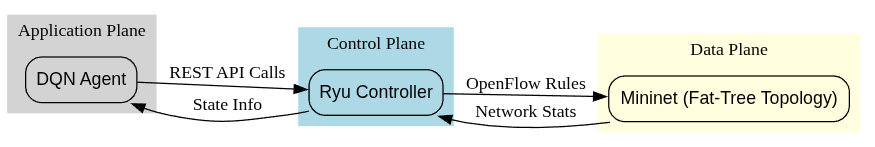
\includegraphics[width=0.8\linewidth]{Images/architecture_placeholder.png}
    \caption{DRL-SDN System Architecture}
\end{figure}
\end{frame}
\begin{frame}{Workflow of the Proposed Approach}
\begin{enumerate}
    \item Collect real-time network and server metrics
    \item Construct state representation
    \item Select action using DQN policy
    \item Enforce policy via OpenFlow rules
    \item Observe reward and next state
    \item Update DQN parameters
\end{enumerate}
\end{frame}
\begin{frame}{Network Topology}
\begin{figure}
    \centering
    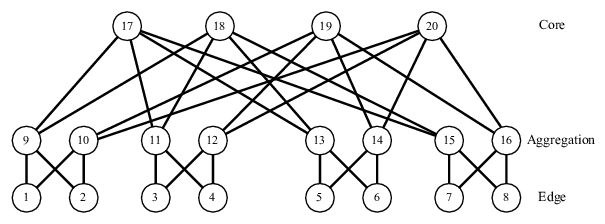
\includegraphics[width=0.75\linewidth]{Images/fat.png}
    \caption{Fat-Tree Topology (k = 4)}
\end{figure}
\end{frame}
\begin{frame}{MDP Formulation}
\begin{itemize}
    \item Problem modeled as Markov Decision Process
    \item Defined by $(\mathcal{S}, \mathcal{A}, \mathcal{R}, \gamma)$
    \item Enables sequential decision-making under uncertainty
\end{itemize}
\end{frame}

% ================= Frame 1: State =================
\begin{frame}{State Space}
\begin{block}{Server Metrics at Time $t$}
The agent observes the following vector of metrics for $S$ backend servers:
\[
\mathbf{s}_t = 
\big[
\text{cpu}_1, \text{memory}_1, \text{rtt}_1, \text{connections}_1, \text{requests}_1, \text{load\_score}_1, \;
\text{cpu}_2, \dots, \text{load\_score}_S
\big]
\]

\begin{itemize}
    \item $\text{cpu}_j$ = CPU usage of server $j$ (0--1)
    \item $\text{memory}_j$ = memory usage of server $j$ (0--1)
    \item $\text{rtt}_j$ = round-trip time to server $j$
    \item $\text{connections}_j$ = number of active connections
    \item $\text{requests}_j$ = total requests handled
    \item $\text{load\_score}_j$ = overall server load (0--1)
\end{itemize}
\end{block}
\end{frame}


% ================= Frame 2: Action =================
\begin{frame}{Action Space}
\begin{block}{Decision per Incoming Flow}
At each time step $t$, the agent selects a backend server for each incoming flow $f$:
\[
a_t : f \mapsto s_j, \quad s_j \in \{1, 2, \dots, S\}
\]

This action decides routing and load distribution across servers.
\end{block}
\end{frame}

% ================= Frame 3: Reward =================
\begin{frame}{Reward Design}
\begin{block}{Objective: Balanced Load and Low Latency}
The reward at time $t$ is computed from real server metrics:
\[
r_t = \underbrace{\alpha e^{- \text{avg RTT}/\tau_\text{RTT}}}_{\text{low latency}}
      + \underbrace{\beta e^{- \text{Var}(\ell_1,\dots,\ell_S)/\tau_\text{var}}}_{\text{balanced load}}
      + \underbrace{\text{balance bonus}}_{\text{even distribution}}
      - \underbrace{\text{overload penalty}}_{\text{avoid overloaded servers}}
\]

\begin{itemize}
    \item $\ell_j$ = server load, $j = 1\dots S$
    \item $\text{avg RTT} = \frac{1}{S}\sum_j rtt_j$
    \item $\text{Var}(\ell_1,\dots,\ell_S)$ = variance of server loads
    \item $\alpha, \beta$ = tunable reward weights
    \item Reward is clipped: $r_t \in [-10, 10]$
\end{itemize}
\end{block}
\end{frame}


\begin{frame}{DRL Agent Design}
\begin{itemize}
    \item Deep Q-Network (DQN)
    \item Online training with replay memory
    \item Target network for stability
    \item $\epsilon$-greedy exploration strategy
\end{itemize}
\end{frame}
\begin{frame}{Training Methodology}
\begin{itemize}
    \item Online interaction with SDN environment
    \item Transition storage in replay buffer
    \item Mini-batch gradient descent updates
    \item Periodic target network synchronization
\end{itemize}
\end{frame}
\begin{frame}{Hyperparameter Configuration}
\begin{itemize}
    \item State dimension: 18
    \item Action dimension: 3
    \item Hidden layer size: 64
    \item Learning rate: $3 \times 10^{-4}$
    \item Discount factor: 0.99
    \item Replay buffer size: 10,000
\end{itemize}
\end{frame}
\begin{frame}{Integration with Ryu Controller}
\begin{itemize}
    \item REST-based agent–controller communication
    \item Collection of port and flow statistics
    \item Dynamic flow rule installation
    \item Closed-loop learning and deployment
\end{itemize}
\end{frame}
\begin{frame}{Evaluation Metrics}
\begin{itemize}
    \item Throughput
    \item End-to-end latency
    \item Jain’s Fairness Index
    \item Link load variance
    \item Server CPU and memory utilization
\end{itemize}
\end{frame}
\begin{frame}{Tools Used}
\begin{itemize}
    \item Ryu Controller, Mininet, Open vSwitch
    \item Python, PyTorch, NumPy, Matplotlib
    \item Iperf, Apache Bench, Wireshark
    \item Arch Linux development environment
\end{itemize}
\end{frame}


\section{Works Completed}
\begin{frame}{System Setup and Environment Configuration}
\begin{itemize}
    \item Linux-based development environment (Arch Linux)
    \item Mininet 2.3.1b4 for network emulation
    \item Ryu controller with Python 3.9 (via pyenv)
    \item Open vSwitch with OpenFlow 1.3 enforced
    \item Controller–switch communication verified on port 6653
\end{itemize}
\end{frame}
\begin{frame}{Environment Verification}
\begin{figure}
    \centering
    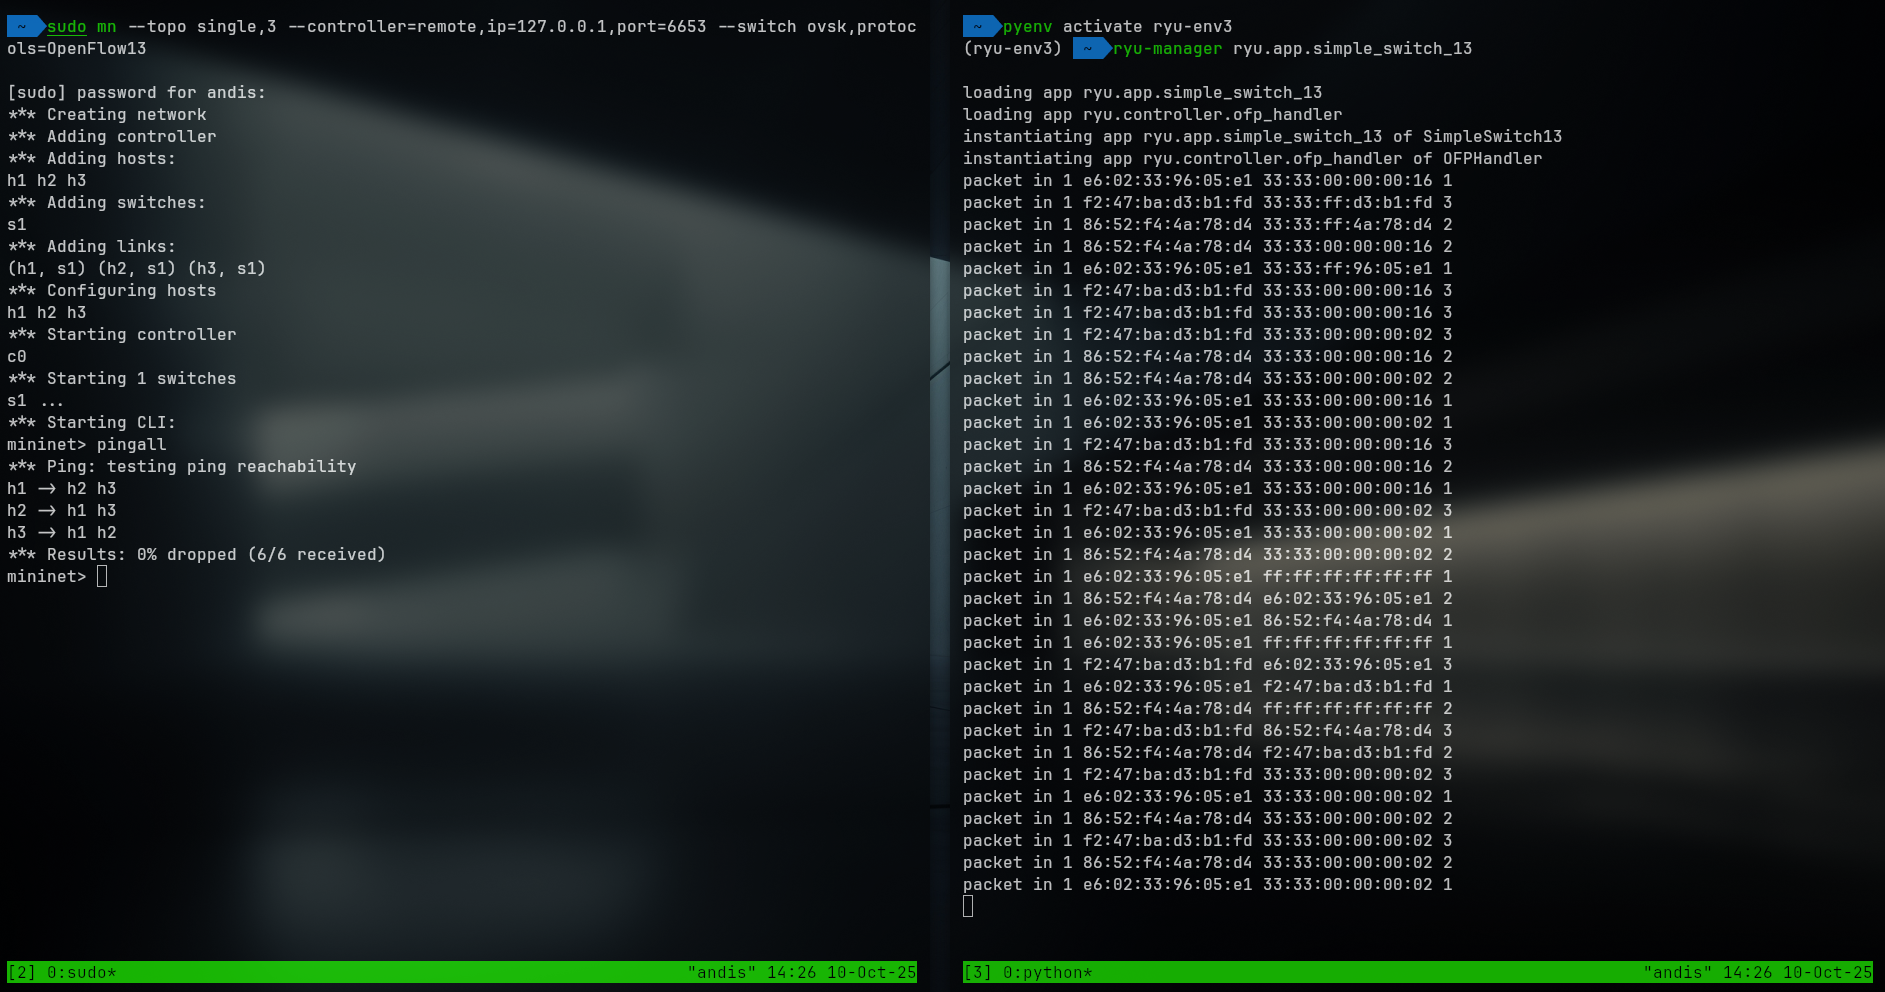
\includegraphics[width=0.7\linewidth]{Images/setup_environment.png}
    \caption{Mininet and Ryu Controller Running Successfully}
\end{figure}
\end{frame}
\begin{frame}{Topology Design and Implementation}
\begin{itemize}
    \item Custom Python script for Fat-Tree topology
    \item Parameter: $k = 4$
    \item Simulates data-center scale network
    \item Hierarchical design: Core, Aggregation, Edge
\end{itemize}
\end{frame}
\begin{frame}{Fat-Tree Topology Structure ($k=4$)}
\begin{itemize}
    \item Core switches: 4
    \item Aggregation switches: 8
    \item Edge switches: 8
    \item Hosts: 16
    \item Designed for high path diversity and scalability
\end{itemize}
\end{frame}
\begin{frame}{Fat-Tree Topology Visualization}
\begin{figure}
    \centering
    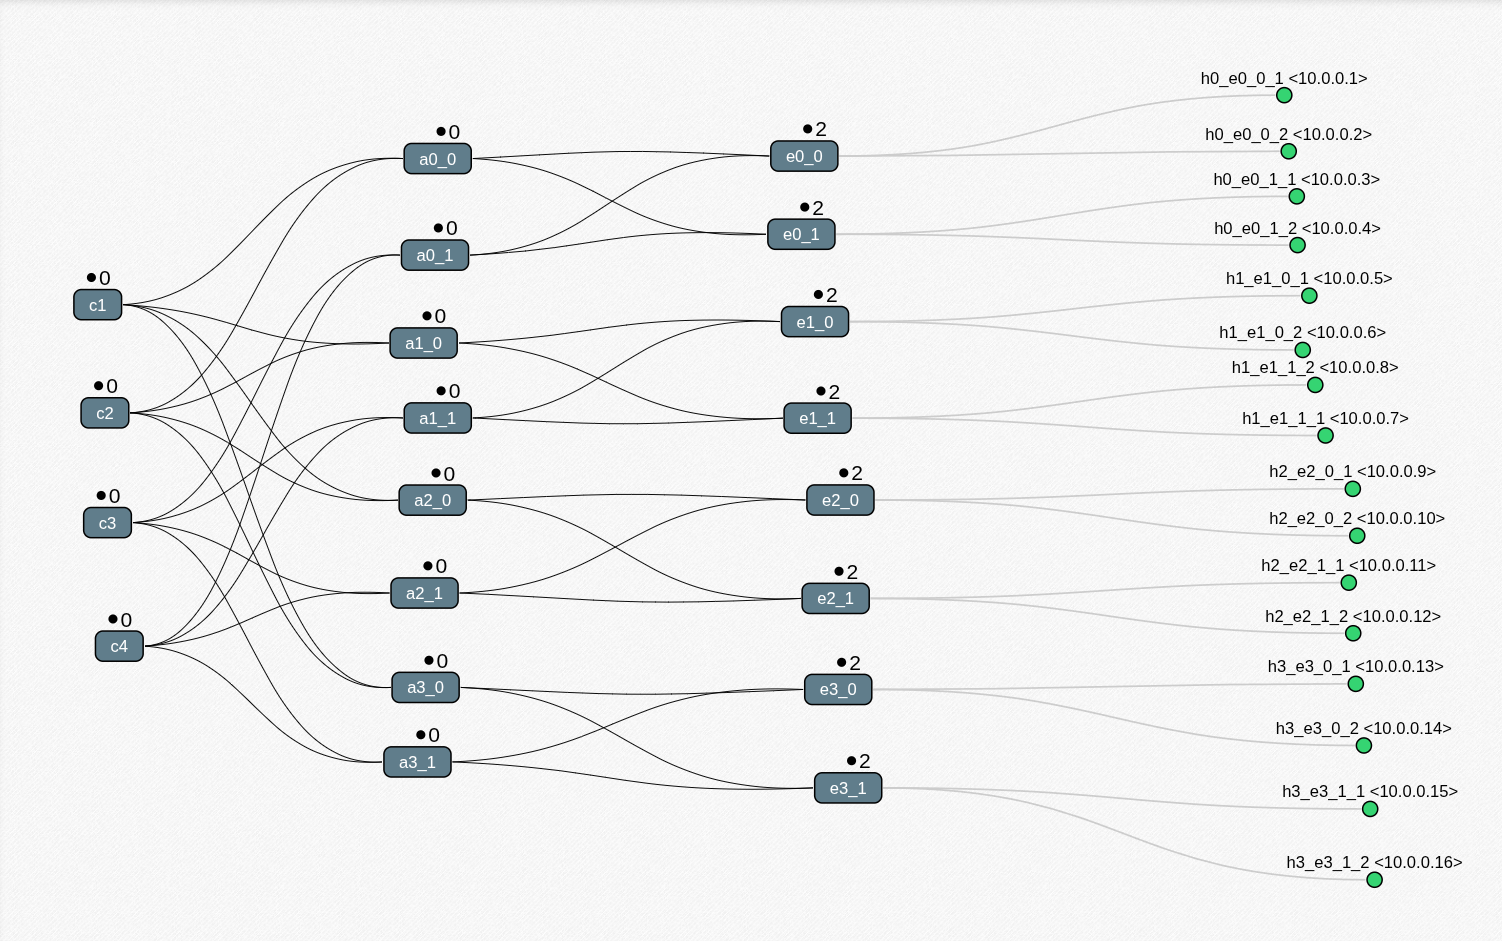
\includegraphics[width=0.7\linewidth]{Images/fat_tree_topology.png}
    \caption{Mininet Fat-Tree Topology ($k=4$)}
\end{figure}
\end{frame}
\begin{frame}{Controller Development}
\begin{itemize}
    \item \textbf{SimpleSwitch13}
    \begin{itemize}
        \item OpenFlow 1.3 learning switch
        \item MAC learning and packet-in handling
    \end{itemize}
    \item \textbf{Enhanced Learning Switch}
    \begin{itemize}
        \item Idle and hard timeouts
        \item LLDP filtering
        \item Precise flow matching
    \end{itemize}
\end{itemize}
\end{frame}
\begin{frame}{Controller Testing and Validation}
\begin{figure}
    \centering
    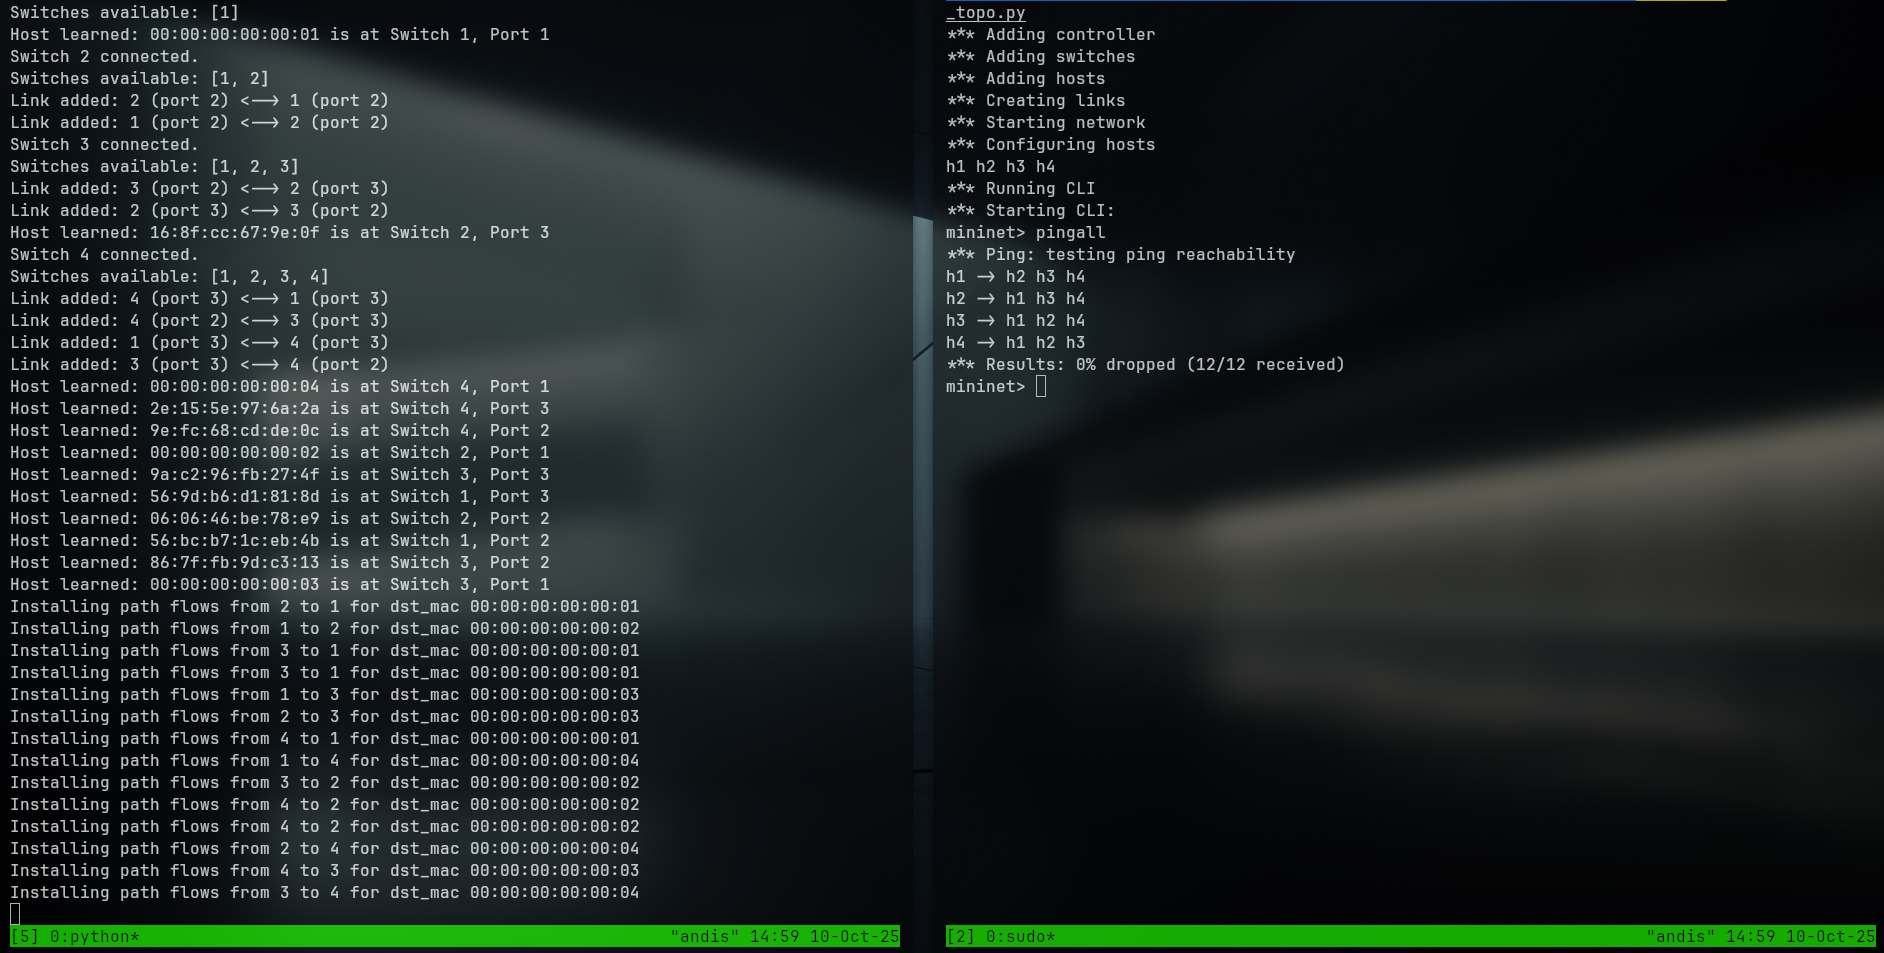
\includegraphics[width=0.7\linewidth]{Images/controller_ping.png}
    \caption{Successful Ping Test in Small SDN Topology}
\end{figure}
\end{frame}
\begin{frame}{Network Monitoring Implementation}
\begin{itemize}
    \item Developed \texttt{NetworkMonitor} Ryu application
    \item Periodic polling of:
    \begin{itemize}
        \item Port statistics
        \item Flow statistics
        \item Packet and byte counters
    \end{itemize}
    \item Enables congestion and utilization analysis
\end{itemize}
\end{frame}
\begin{frame}{Real-Time Monitoring Output}
\begin{figure}
    \centering
    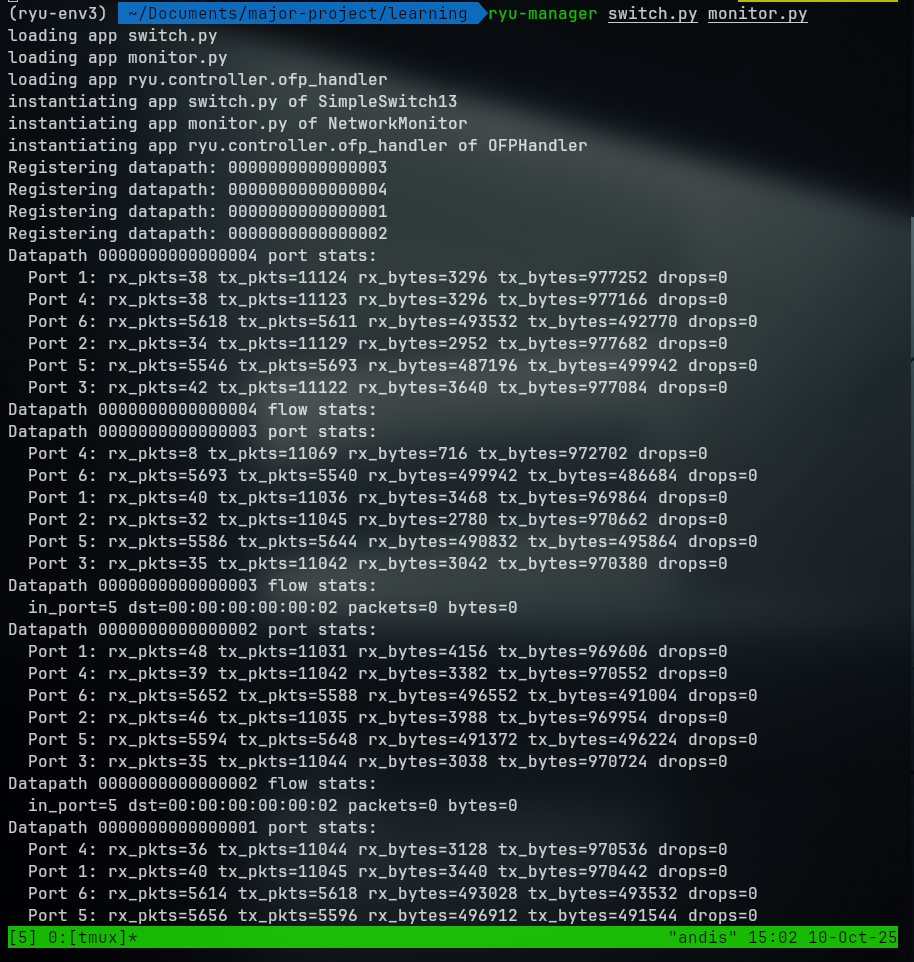
\includegraphics[width=0.7\linewidth]{Images/network_monitor.png}
    \caption{Live Port and Flow Statistics Collection}
\end{figure}
\end{frame}
\begin{frame}{Traffic Generation Setup}
\begin{itemize}
    \item ApacheBench used for realistic client behavior
    \item Traffic patterns:
    \begin{itemize}
        \item Constant
        \item Bursty
        \item Incremental
    \end{itemize}
    \item Enables stress-testing of load balancer
\end{itemize}
\end{frame}
\begin{frame}{Traffic Patterns}
\begin{figure}
    \centering
    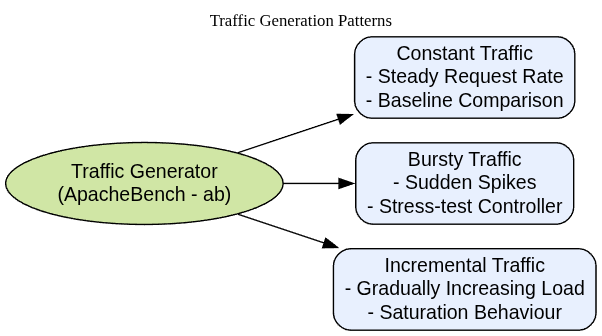
\includegraphics[width=0.7\linewidth]{Images/traffic_patterns_placeholder.png}
    \caption{Traffic Load Patterns Used for Training}
\end{figure}
\end{frame}
\begin{frame}{Controller Initialization}
\begin{itemize}
    \item Virtual IP successfully registered
    \item Backend server pool initialized (h1, h2, h3)
\end{itemize}

\begin{figure}
    \centering
    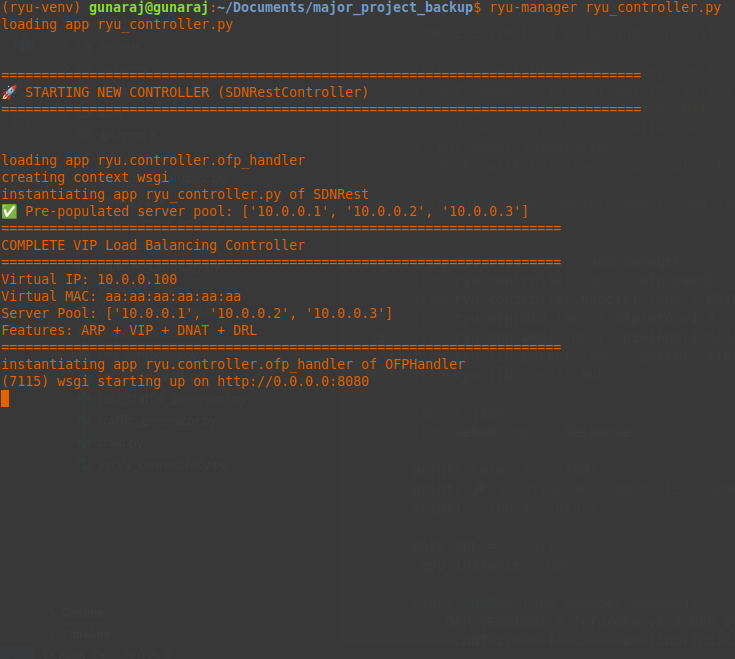
\includegraphics[width=0.6\linewidth]{Images/init.png}
    \caption{Controller Initialization Logs}
\end{figure}
\end{frame}
\begin{frame}{Routing Installation}
\begin{itemize}
    \item Static routing used for baseline connectivity
    \item 921 flow rules installed
    \item Ensures full reachability before DRL decisions
\end{itemize}

\begin{figure}
    \centering
    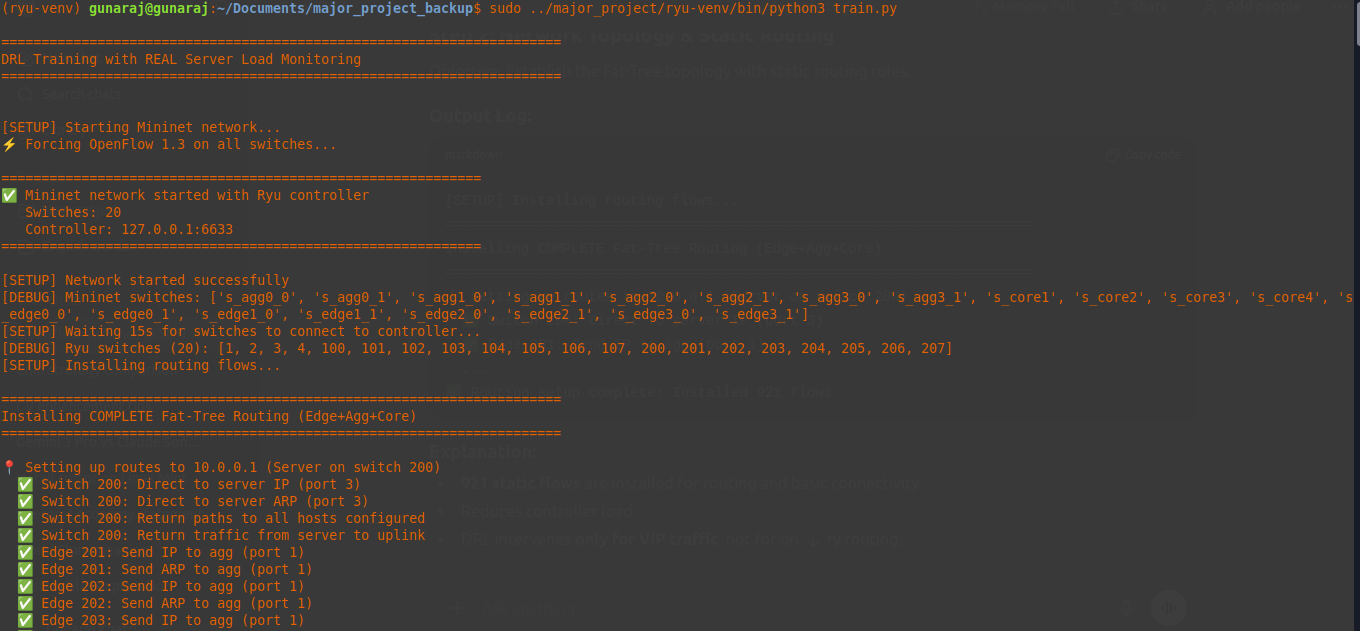
\includegraphics[width=0.6\linewidth]{Images/route_init.png}
    \caption{Static Routing Initialization}
\end{figure}
\end{frame}
\begin{frame}{Real-Time DRL Decision Making}
\begin{itemize}
    \item DRL agent selects server per request
    \item Decisions based on real-time metrics
    \item Integrated with Ryu via REST APIs
\end{itemize}

\begin{figure}
    \centering
    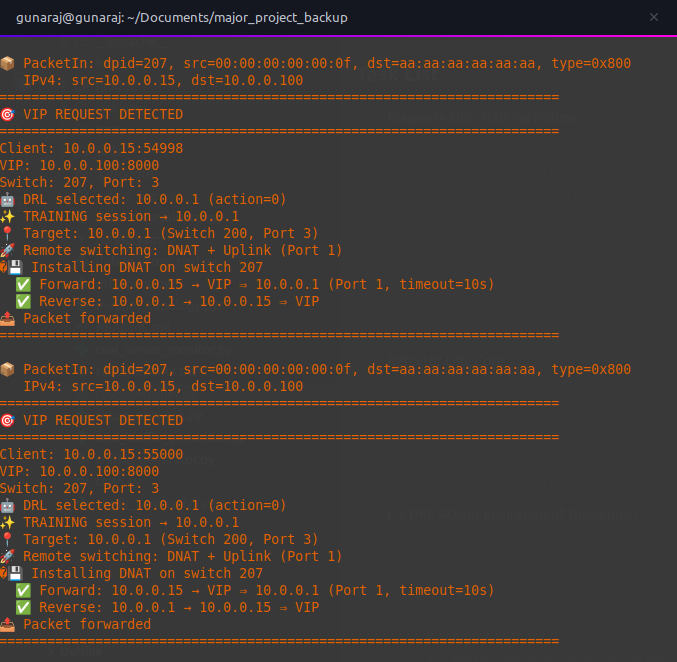
\includegraphics[width=0.5\linewidth]{Images/drl.png}
    \caption{DRL Agent Decision Logs}
\end{figure}
\end{frame}


% ================= Q LEARNING =================
\begin{frame}{Neural Network Implementation}

\begin{figure}
    \centering
    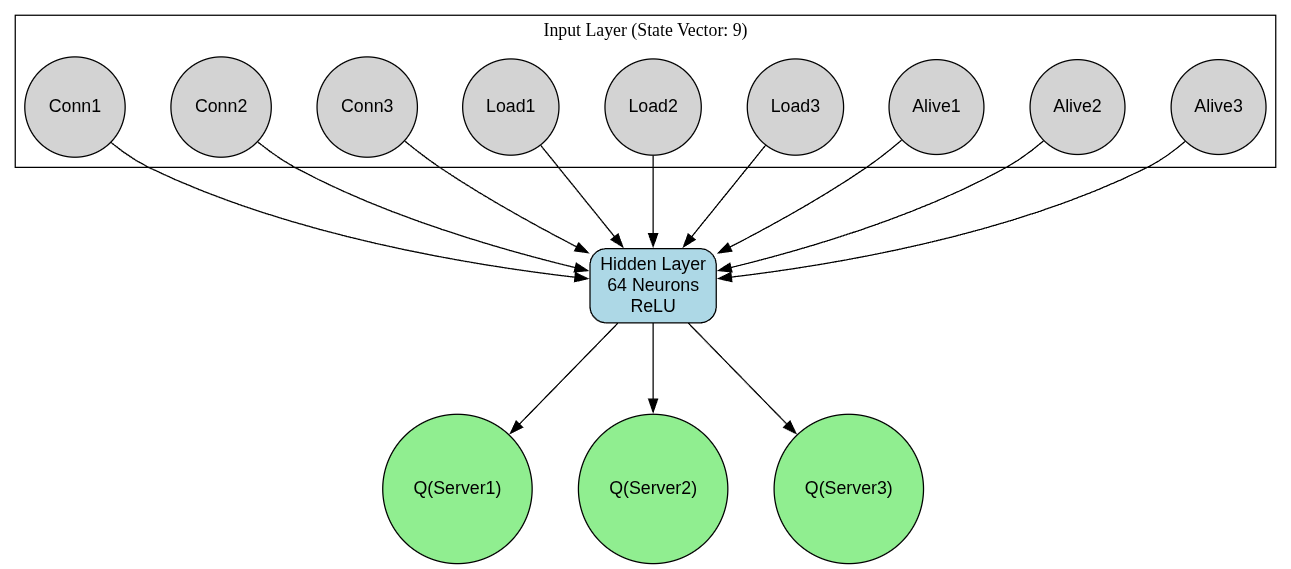
\includegraphics[width=0.75\linewidth]{Images/neuralnet.png}
    \caption{Neural Network}
\end{figure}
\end{frame}

% ================= SYSTEM INTEGRATION =================

\begin{frame}{System Integration}
\begin{figure}
    \centering
    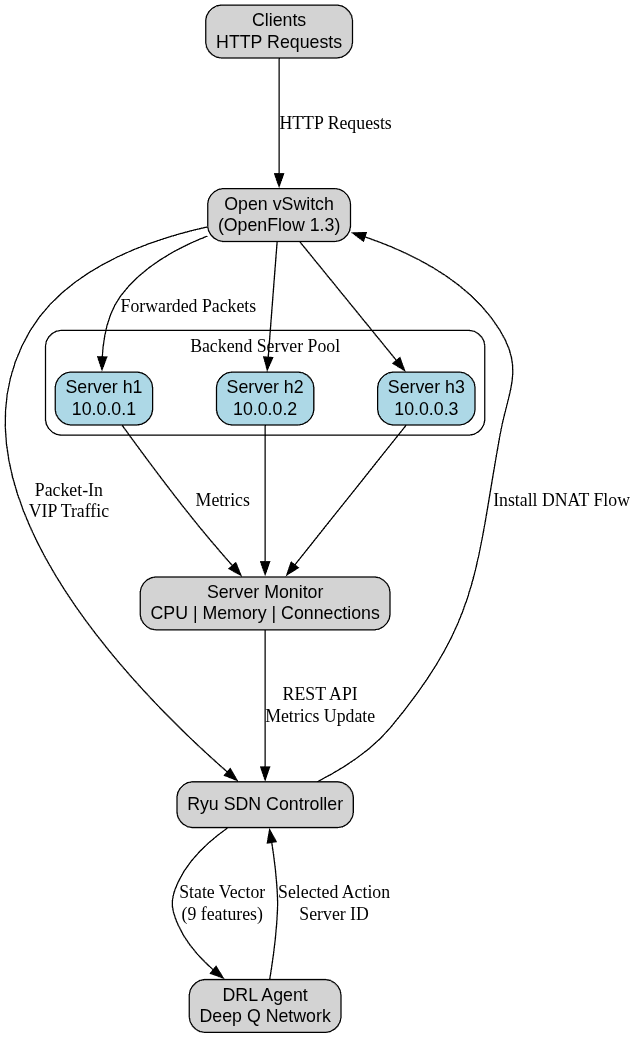
\includegraphics[width=0.25\linewidth]{Images/arch.png}
    \caption{DRL-SDN System Architecture}
\end{figure}
\end{frame}

% ================= TRAINING METRICS =================
\begin{frame}{Training Metrics}

\begin{figure}
    \centering
    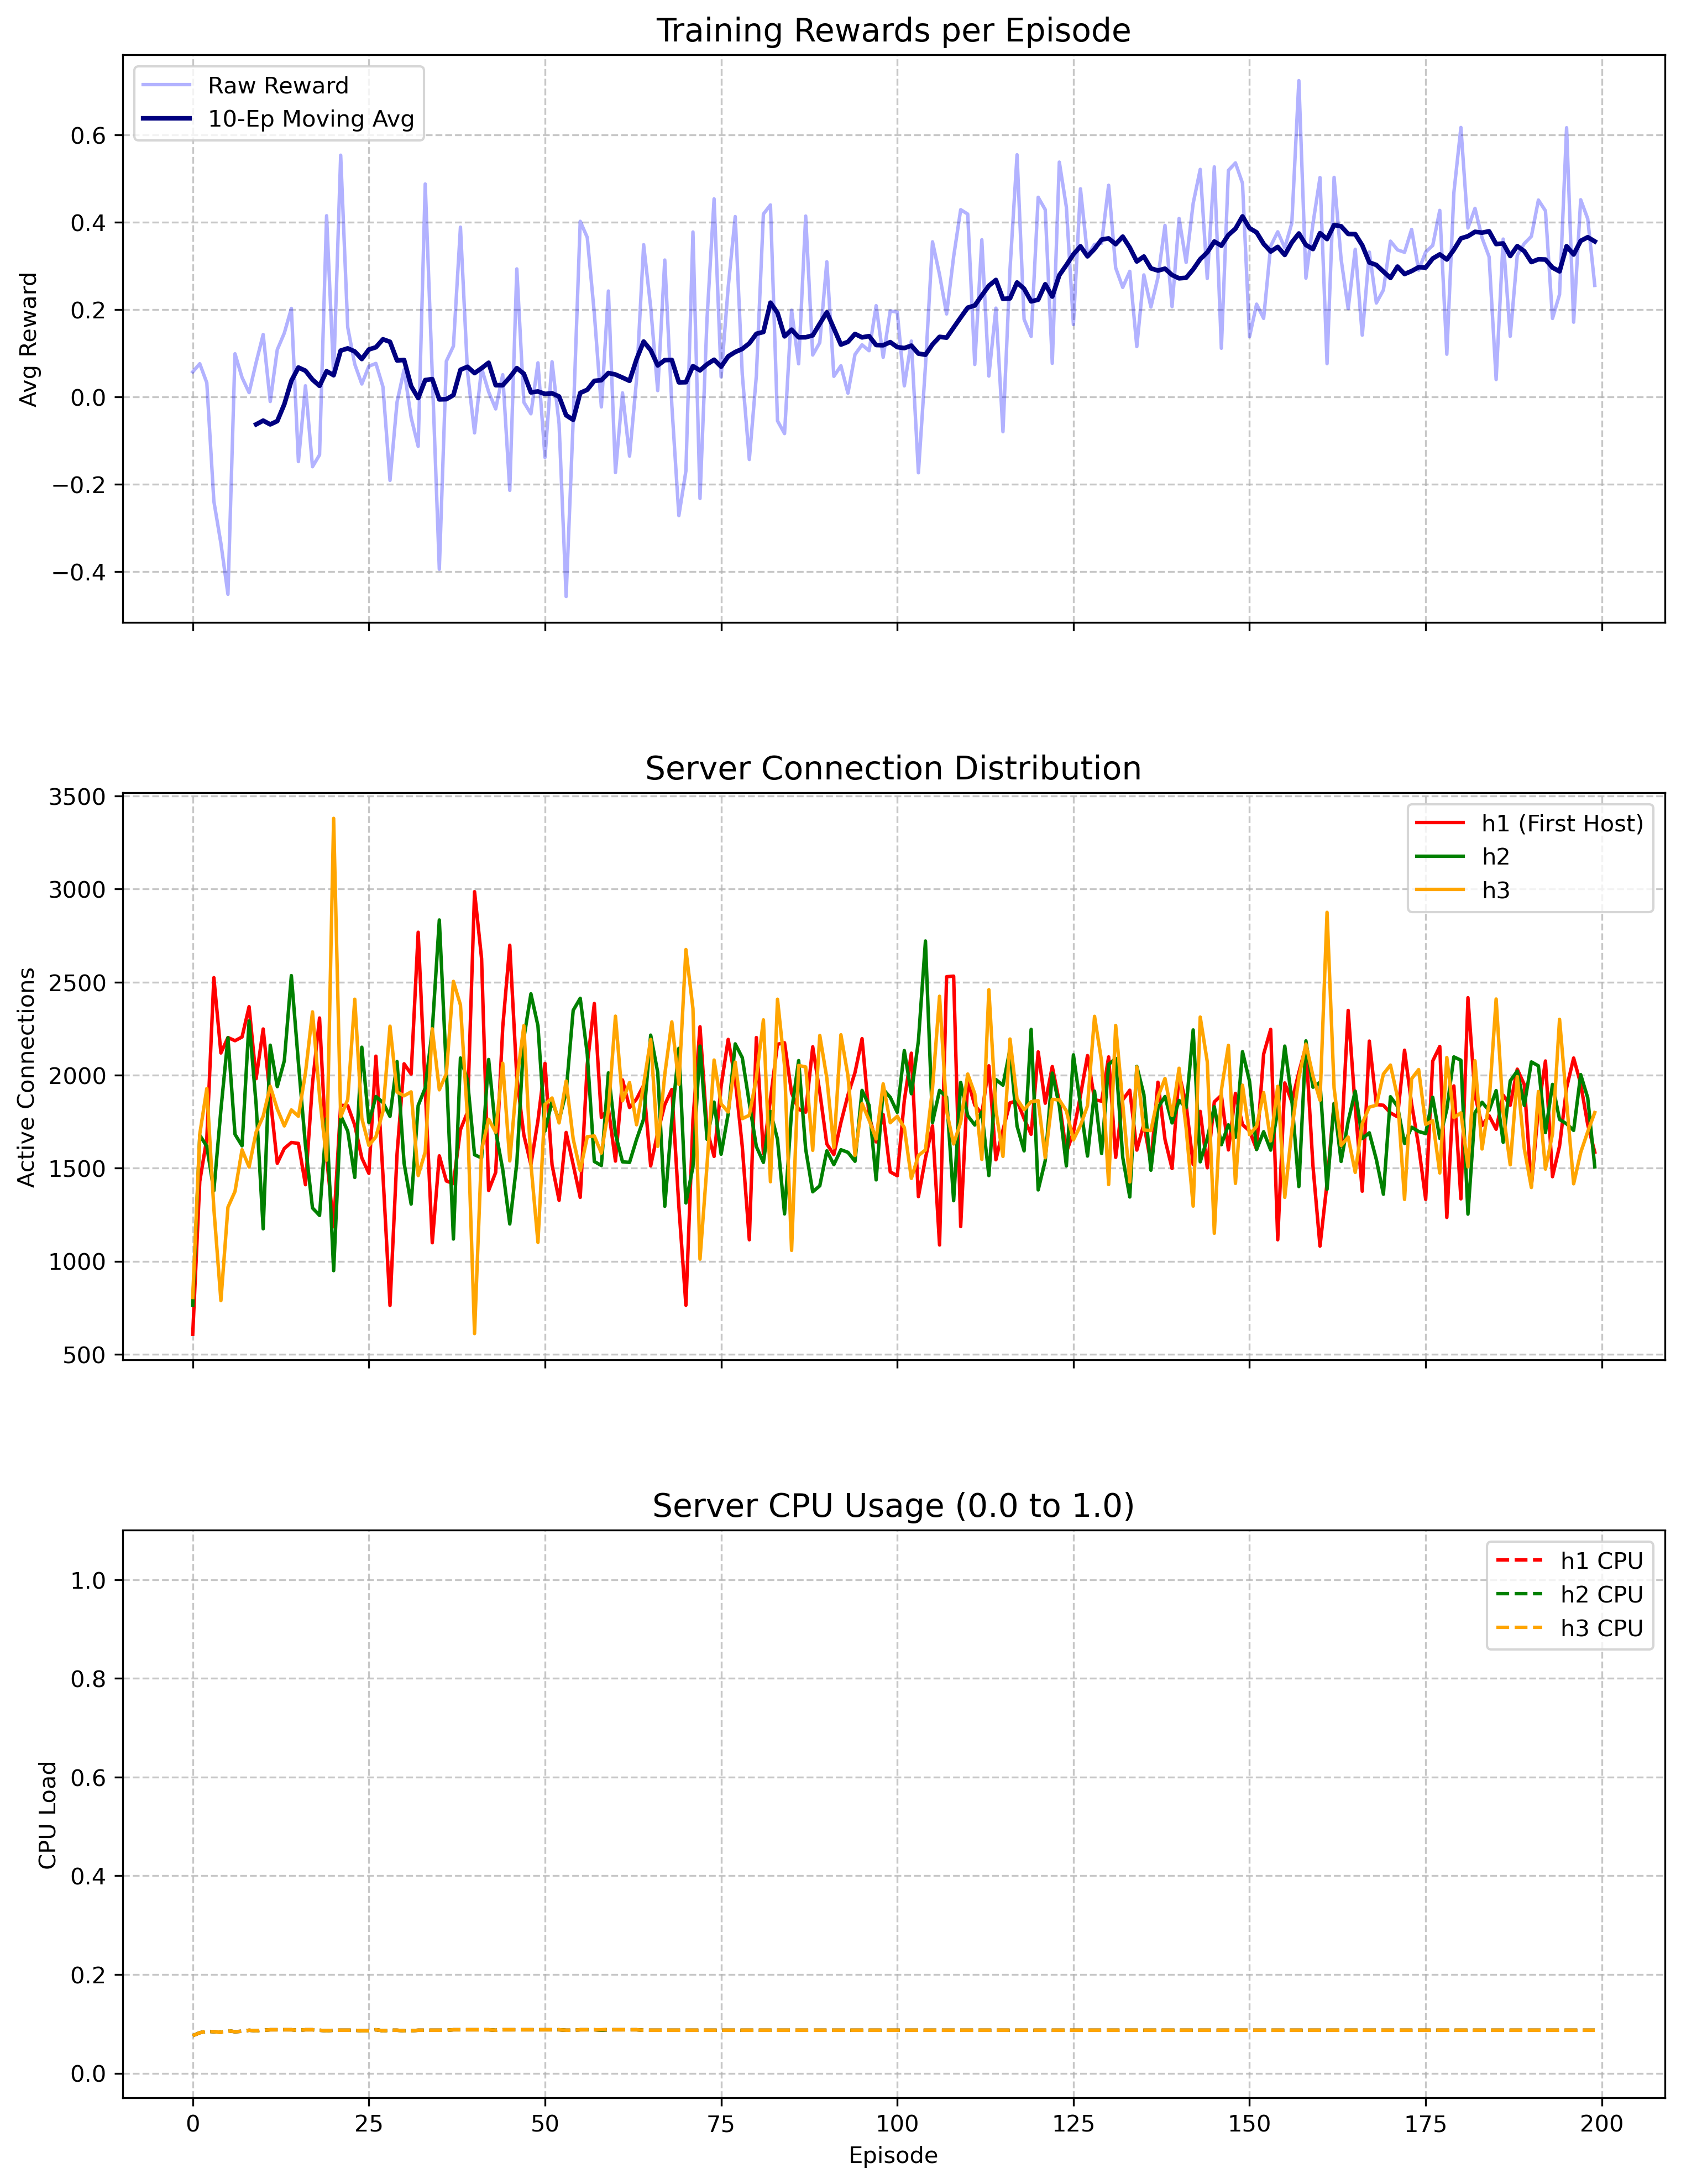
\includegraphics[width=0.55\linewidth]{Images/training_summary.png}
    \caption{Training Metrics Over Episodes}
\end{figure}
\end{frame}

% ================= CHECKPOINTING =================
\begin{frame}{Model Checkpointing}
\begin{itemize}
    \item Model saved every 10 episodes
    \item Evaluation run every 20 episodes ($\epsilon=0$)
    \item Final model stored after training
    \item Logs saved as JSON for analysis
\end{itemize}
\end{frame}

% ================= INFERENCE =================
\begin{frame}{Inference Mode (Evaluation)}
\begin{itemize}
    \item Exploration disabled ($\epsilon = 0$)
    \item Agent acts purely on learned policy
    \item Traffic: 80 requests/sec for 120 seconds
    \item System polled every second
\end{itemize}
\end{frame}

% ================= INFERENCE RESULTS =================
\begin{frame}{Inference Results}
\begin{figure}
    \centering
    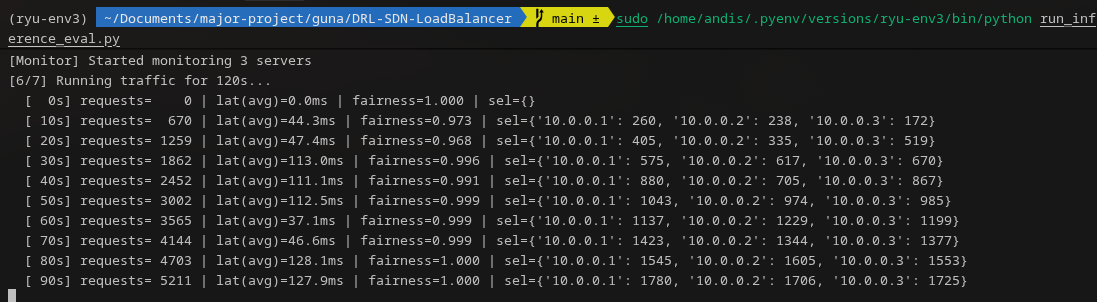
\includegraphics[width=0.85\linewidth]{Images/inference.png}
    \caption{Evaluation Output}
\end{figure}
\end{frame}

\begin{frame}{Inference Results}
\begin{figure}
    \centering
    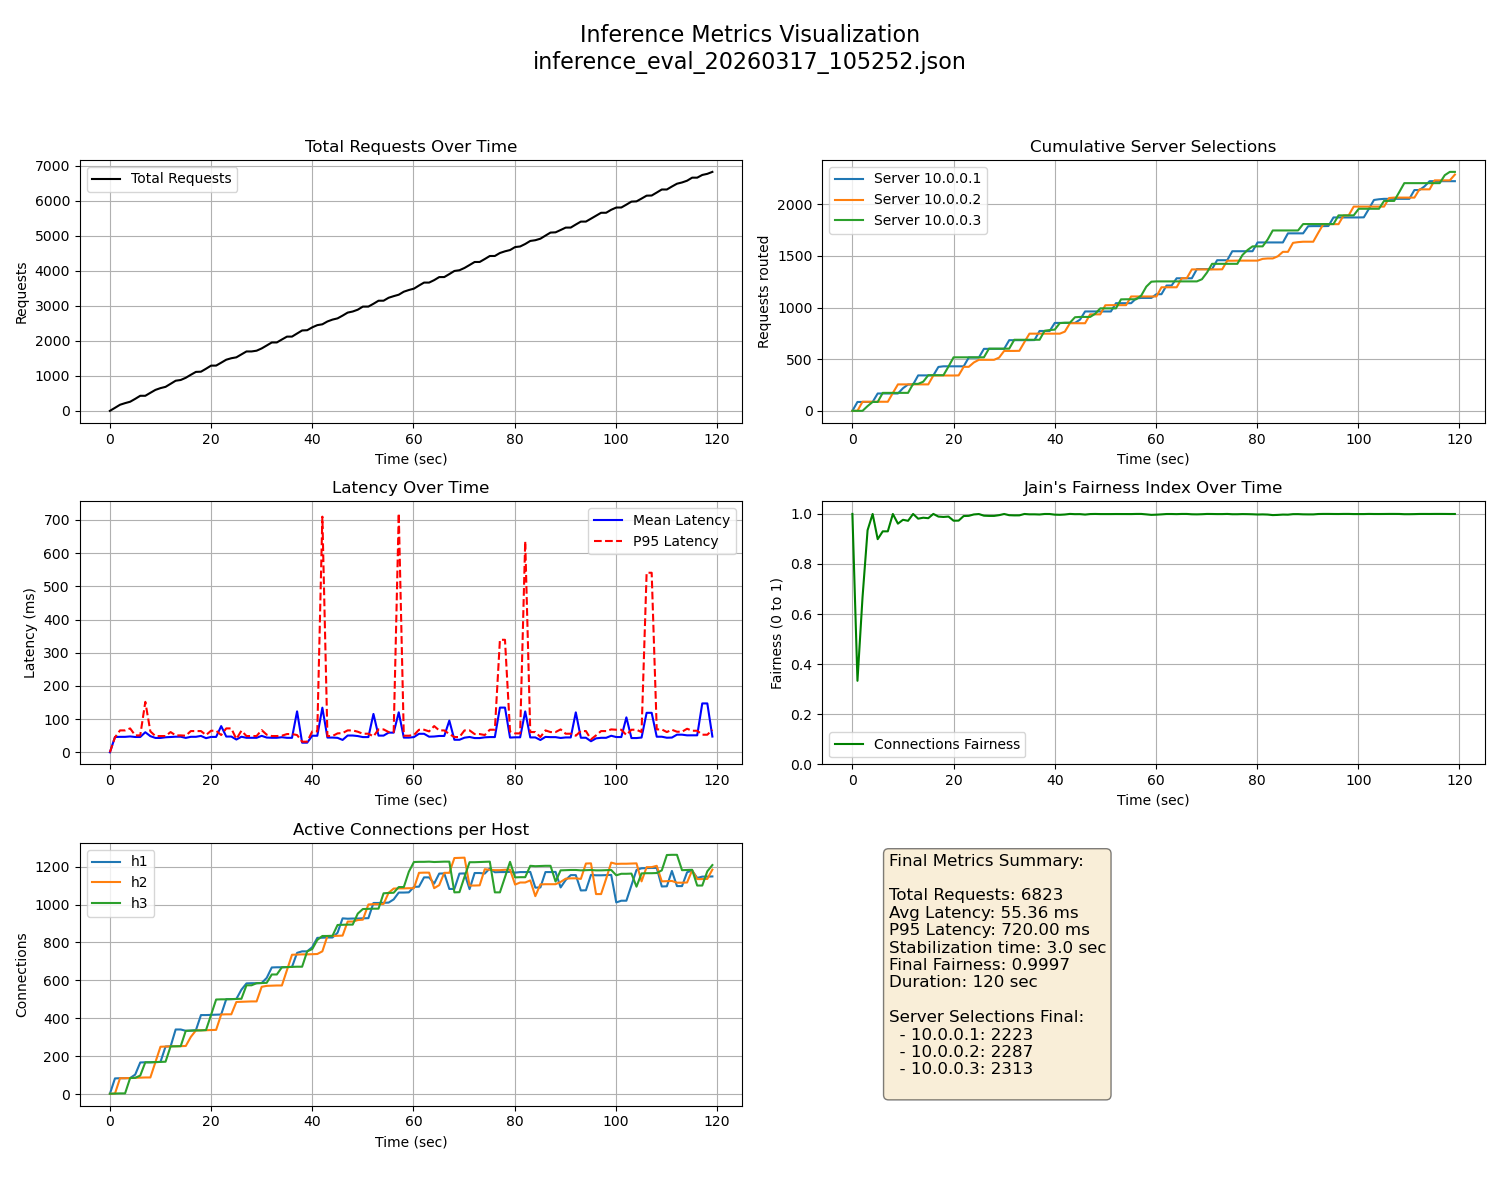
\includegraphics[width=0.85\linewidth]{Images/inference_plot.png}
    \caption{Results During Evaluation}
\end{figure}
\end{frame}



% ================= OBSERVATIONS =================
\begin{frame}{Observations}
\begin{itemize}
    \item Agent learns near-uniform load distribution
    \item Reward stabilizes across episodes
    \item Latency improves compared to naive routing
    \item System adapts to traffic variations
\end{itemize}
\end{frame}

% ================= LIMITATIONS =================
\begin{frame}{Current Limitations}
\begin{itemize}
    \item Simulation-only evaluation using Mininet
    \item Single SDN controller (Ryu)
    \item Synthetic traffic generation (Apache Bench)
    \item No deployment on real SDN hardware
    \item Small-scale topology (3 servers)
    \item Delays in metric collection
    \item Hyperparameter sensitivity
    \item Mininet lacks hardware-level realism
\end{itemize}
\end{frame}


% ================= SUMMARY =================
\begin{frame}{Summary of Accomplishments}
\begin{itemize}
    \item Complete DRL-SDN pipeline implemented
    \item MDP formulation and DQN training completed
    \item Real traffic-based training executed
    \item Inference evaluation with fairness and latency metrics
    \item System ready for benchmarking and scaling
\end{itemize}
\end{frame}


% \section{Work Remaining}
\begin{frame}{Refinement of Load Balancing Mechanism}
\begin{itemize}
    \item Path-aware shortest-path computation across SDN switches
    \item End-to-end flow management with IP/MAC rewriting for VIP traffic
    \item Enhanced real-time server health monitoring
\end{itemize}
\end{frame}
\begin{frame}{Planned Load Balancing Design}
\begin{figure}
    \centering
    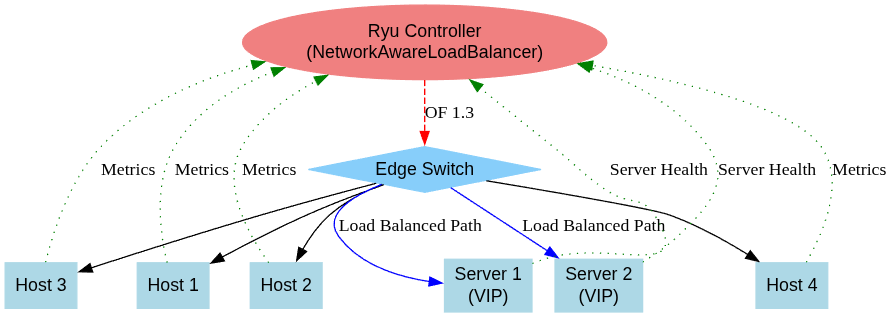
\includegraphics[width=\linewidth]{Images/load_balancing_design.png}
    \caption{Planned SDN Load Balancing Workflow}
\end{figure}
\end{frame}
\begin{frame}{Refinement of DRL-Based Approach}
\begin{itemize}
    \item Extended training for convergence validation (200+ episodes)
    \item Hyperparameter fine-tuning for stability
    \item Comparison with traditional load balancing algorithms
\end{itemize}
\end{frame}
\begin{frame}{Planned Baseline Comparison}
\begin{itemize}
    \item Round-Robin load balancing
    \item Static shortest-path routing
    \item DRL-based intelligent load balancing
\end{itemize}
\end{frame}
\begin{frame}{Simulation and Performance Evaluation}
\begin{itemize}
    \item Controlled simulation under diverse traffic patterns
    \item Metrics for evaluation:
    \begin{itemize}
        \item Throughput
        \item End-to-end latency
        \item Packet loss
        \item Server utilization
    \end{itemize}
    \item Statistical and graphical comparison
\end{itemize}
\end{frame}
\begin{frame}{Documentation and Final Deliverables}
\begin{itemize}
    \item Comprehensive experimental documentation
    \item Final project report preparation
    \item Final defense presentation
\end{itemize}
\end{frame}
\begin{frame}{Overall Project Workflow and Next Steps}
\begin{figure}
    \centering
    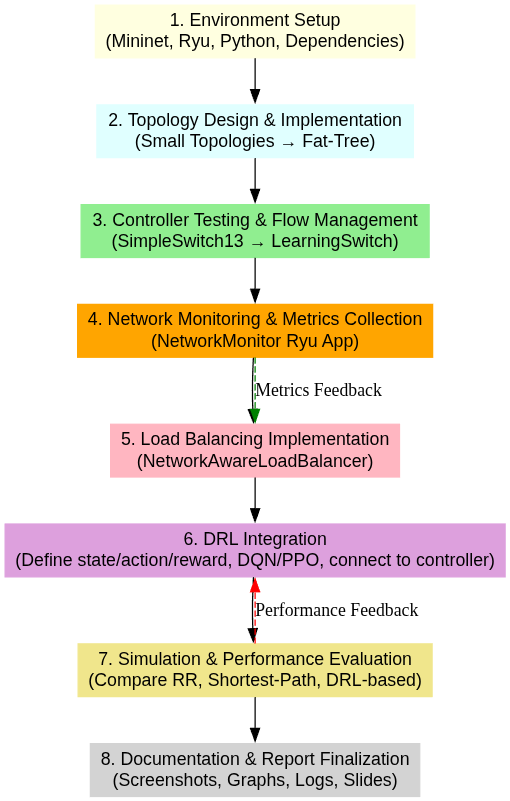
\includegraphics[width=0.3\linewidth]{Images/project_workflow.png}
    \caption{End-to-End Project Workflow}
\end{figure}
\end{frame}
\begin{frame}{Mid-Term Status Summary}
\begin{itemize}
    \item Core SDN and DRL framework implemented
    \item System is fully functional end-to-end
    \item Remaining work focuses on refinement and evaluation
    \item No major architectural risks remaining
\end{itemize}
\end{frame}

\section*{Q \& A}
\begin{frame}{Thank You}
  \centering
  \Large We humbly ask for your suggestions.
\end{frame}

\end{document}
